\documentclass[a4paper,12pt]{article}

\usepackage{graphicx}
\usepackage{caption}
\usepackage{subcaption}
\usepackage{tikz}
\usepackage{pgf}
\usepackage{amsmath}
\usetikzlibrary{arrows.meta}
\usepackage[utf8]{inputenc}
\usepackage[english,greek]{babel}
\usepackage{hyperref}

\title{Προσομοίωση και Μοντελοποίηση \newline Δυναμικών Συστημάτων \newline Εργασία 1}
\author{Ρουσομάνης Γεώργιος (ΑΕΜ: 10703)}
\date{Μάρτιος 2025}

\begin{document}

\maketitle

\section*{Εισαγωγή}


\section*{Θέμα 1}
Το υπό μελέτη σύστημα πρόκειται για ένα απλό εκκρεμές με ροπή εισόδου, το οποίο περιγράφεται, έπειτα από γραμμικοποίηση ($sin(q) \approx q$ για μικρές γωνίες $q$), από τη διαφορική εξίσωση:
\begin{equation}
    mL^2\ddot{q}(t) + c\dot{q}(t) + mgLq(t) = u(t),
    \label{eq:system_differential_equation}
\end{equation}
όπου $q(t)$ \selectlanguage{english}[rad]\selectlanguage{greek} η γωνία εκτροπής του εκκρεμούς, 
$m$ \selectlanguage{english}[kg]\selectlanguage{greek}, $L$ \selectlanguage{english}[m]\selectlanguage{greek} 
η μάζα και το μήκος του εκκρεμούς, αντίστοιχα, $c$ \selectlanguage{english}[N $\cdot$ m $\cdot$ sec]\selectlanguage{greek} 
ένας σταθερός συντελεστής απόσβεσης, $g$ \selectlanguage{english}[m/sec$^2$]\selectlanguage{greek} η
επιτάχυνση της βαρύτητας, και $u(t)$ \selectlanguage{english}[N $\cdot$ m]\selectlanguage{greek} η είσοδος ελέγχου.

\subsection*{Ερώτημα 1α}
Η παραπάνω διαφορική εξίσωση περιγράφει ένα Γραμμικό και Χρονικά Αμετάβλητο Σύστημα (ΓΧΑ), συνεπώς το σύστημα μπορεί
να περιγραφεί ισοδύναμα από ένα σύνολο διαφορικών εξισώσεων της μορφής:
\begin{equation}
\begin{aligned}
    \dot{x}(t) &= A x(t) + B u(t) \\
    y(t) &= C x(t) + D u(t)
\end{aligned}
\label{eq:system_states}
\end{equation}
όπου $x(t)$ το διάνυσμα κατάστασης και $y$ η έξοδος του συστήματος. Η (\ref{eq:system_states}) αποτελεί τις εξισώσεις
κατάστασης του συστήματος. 

Για να φέρουμε το σύστημα στην παραπάνω μορφή, ακολουθούμε την εξής διαδικασία.
Από την (\ref{eq:system_differential_equation}) έχουμε:
\begin{equation}
    \ddot{q}(t) = -\frac{c}{mL^2}\dot{q}(t) -\frac{g}{L}q(t) +\frac{1}{mL^2} u(t).
    \label{eq:system_differential_equation2}
\end{equation}
Θέτοντας $x_1 = q(t)$ και $x_2 = \dot{q}(t) = \dot{x}_1$ παίρνουμε $\ddot{q}(t) = \dot{x}_2$ και προκύπτει το σύστημα:
\begin{equation}
\begin{aligned}
    \dot{x}_1 &= x_2 \\
    \dot{x}_2 &= -\frac{c}{mL^2}x_2 -\frac{g}{L}x_1 +\frac{1}{mL^2} u(t).
    \label{eq:system_states2}
\end{aligned}
\end{equation}
Θεωρώντας ως έξοδο $y$ του συστήματος την γωνία εκτροπής του εκκρεμούς $q$, οι εξισώσεις κατάστασης του συστήματος
δίνονται από: 
\begin{equation}
\begin{aligned}
    \left[
    \begin{matrix}
        \dot{x}_1 \\
        \dot{x}_2
    \end{matrix}
    \right]
    &=
    \left[
    \begin{matrix}
        0 & 1 \\
        -\frac{g}{L} & -\frac{c}{mL^2}
    \end{matrix}
    \right]
    \cdot
    \left[
    \begin{matrix}
        x_1 \\
        x_2
    \end{matrix}
    \right]
    +
    \left[
    \begin{matrix}
        0 \\
        \frac{1}{mL^2}
    \end{matrix}
    \right]
    u(t)
    \\
    y &= 
    \left[
    \begin{matrix}
        1 & 0
    \end{matrix}
    \right]
    \cdot
    \left[
    \begin{matrix}
        x_1 \\
        x_2
    \end{matrix}
    \right]
    \label{eq:system_states_final}
\end{aligned}
\end{equation}
Συγκρίνοντας τις (\ref{eq:system_states}), (\ref{eq:system_states_final}) προκύπτει
\begin{equation}
    A = 
    \left[
    \begin{matrix}
        0 & 1 \\
        -\frac{g}{L} & -\frac{c}{mL^2}
    \end{matrix}
    \right], \quad
    B = 
    \left[
    \begin{matrix}
        0 \\
        \frac{1}{mL^2}
    \end{matrix}
    \right], \quad
    C = 
    \left[
    \begin{matrix}
        1 & 0
    \end{matrix}
    \right], \quad
    D = 0
    \label{eq:system_states_matrices}
\end{equation}

Η συνάρτηση μεταφοράς μπορεί εύκολα να υπολογιστεί από τον τύπο:
\begin{equation}
    H(s) = C (sI-A)^{-1}B + D,
    \label{eq:transfer_function_formula}
\end{equation}
και με αντικατάσταση των πινάκων από την (\ref{eq:system_states_matrices}), βρίσκουμε:
\begin{equation}
    H(s) = \frac{1}{mL^2s^2 + cs + mgL}.
    \label{eq:transfer_function}
\end{equation}

\subsection*{Ερώτημα 1β}
Για να προσομοιώσουμε την απόκριση του συστήματος πρέπει αρχικά να προσδιορίσουμε αν το σύστημά μας είναι άκαμπτο ή 
μη άκαμπτο ώστε να επιλέξουμε την κατάλληλη συνάρτηση \selectlanguage{english}ODE solver\selectlanguage{greek} του 
\selectlanguage{english}MATLAB\selectlanguage{greek}.

Αντικαθιστώντας τις τιμές $m = 0.75, L = 1.25, c = 0.15, g = 9.81$ στην (\ref{eq:transfer_function}) και παίρνοντας 
τον αντίστροφο Μ/Σ \selectlanguage{english}Laplace\selectlanguage{greek} βρίσκουμε τους πόλους της συνάρτησης μεταφοράς
$-0.064\pm2.8i$. Παρατηρούμε ότι το σύστημά μας είναι ευσταθές καθώς οι πόλοι της συνάρτησης μεταφοράς βρίσκονται στο 
αριστερό ημιεπίπεδο. Επίσης οι σταθερές χρόνου των δύο πόλων ταυτίζονται $\tau=0.064$ καθως είναι συζυγείς μιγαδικοί, 
επμένως είναι της ίδιας τάξης μεγέθους και το σύστημά μας είναι μη άκαμπτο. Μία καλή επιλογή 
\selectlanguage{english}ODE solver\selectlanguage{greek} στο \selectlanguage{english}MATLAB\selectlanguage{greek} 
για μη άκαμπτα συστήματα είναι η συνάρτηση \selectlanguage{english}ode45\selectlanguage{greek} την οποία και 
χρησιμοποιούμε στην ανάλυσή μας.

Στο Σχ.~\ref{fig:task1_system_response} βλέπουμε την έξοδο του συστήματος και την παράγωγό της για είσοδο 
$u(t) = A_0 sin(\omega t)$ με $A_0 = 4, \, \omega = 2$ και βήμα ολοκλήρωσης $\Delta t = 10^{-3}$
\selectlanguage{english}[sec]\selectlanguage{greek} ενώ στο Σχ.~\ref{fig:task1_system_states} παρατίθεται το 
αντιστοιχο διάγραμμα καταστάσεων.

\begin{figure}[!h]
    \centering
    \begin{minipage}{0.45\textwidth}
        \centering
        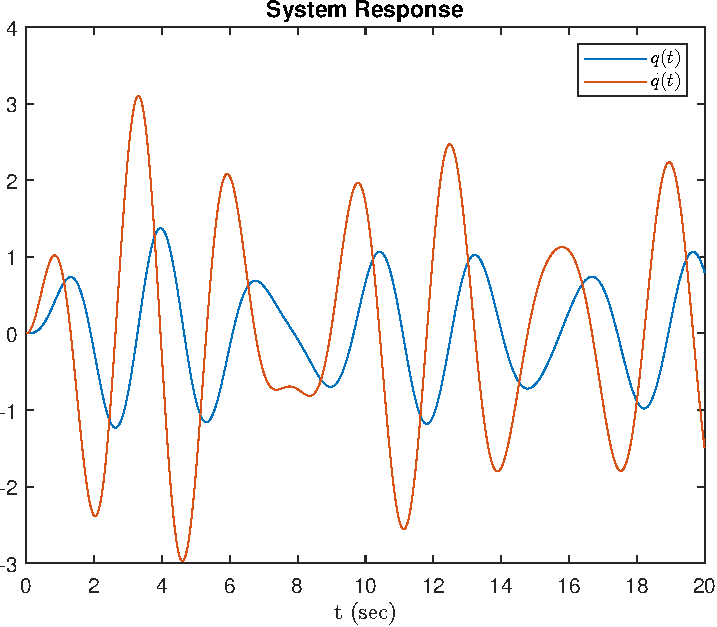
\includegraphics[width=\linewidth]{plot/task1_system_response.pdf}
        \caption{Απόκριση του συστήματος για βήμα ολοκλήρωσης $\Delta t = 10^{-3}$ 
        \selectlanguage{english}[sec]\selectlanguage{greek}}
        \label{fig:task1_system_response}
    \end{minipage}
    \hfill
    \begin{minipage}{0.45\textwidth}
        \centering
        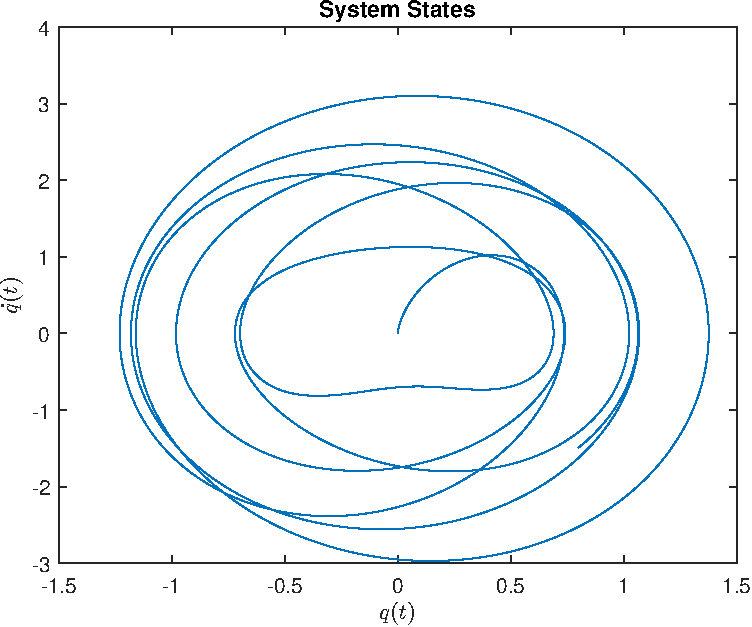
\includegraphics[width=\linewidth]{plot/task1_system_states.pdf}
        \caption{Γράφημα καταστάσεων του συστήματος για χρόνο προσομοίωσης 20 
        \selectlanguage{english}[sec]\selectlanguage{greek}}
        \label{fig:task1_system_states}
    \end{minipage}
\end{figure}

\section*{Θέμα 2}
\subsection*{Ερώτημα 2α}
Θα εκτιμήσουμε τις παραμέτρους $m, L, c$ του συστήματος χρησιμοποιώντας την μέθοδο των ελαχίστων τετραγώνων, 
θεωρώντας μετρήσιμα τα $q(t), \dot{q}(t)$ καθώς και την είσοδο $u(t)$. Για να το επιτύχουμε αυτό, πρέπει αρχικά 
να φέρουμε το σύστημά μας στην γραμμική παραμετροποιήσιμη μορφή. Η (\ref{eq:system_differential_equation2}) μπορεί 
να γραφεί στη μορφή:
\begin{equation}
    \ddot{q} =
    \left[
    \begin{matrix}
        \frac{c}{mL^2} & \frac{g}{L} & \frac{1}{mL^2}
    \end{matrix}
    \right]
    \cdot
    \left[
    \begin{matrix}
        -\dot{q} & -q & u
    \end{matrix}
    \right]^T
    \label{eq:linear_parametric_form}
\end{equation}
Στην παραπάνω σχέση το $\ddot{q}$ δεν είναι μετρίσιμο, συνεπώς η εκτίμηση των παραμέτρων δεν είναι εφικτή.
Για να ξεπεράσουμε αυτό το πρόβλημα, θέτουμε $\ddot{q} = s\dot{q}$ και φιλτράρουμε τα δύο μέλη της 
(\ref{eq:linear_parametric_form}) με ένα ευσταθές φίλτρο $\Lambda(s) = s + \lambda$. Επομένως η 
(\ref{eq:linear_parametric_form}) γίνεται:
\begin{equation}
\begin{aligned}
    \frac{s}{\Lambda(s)}\dot{q} &=
    \left[
    \begin{matrix}
        \frac{c}{mL^2} & \frac{g}{L} & \frac{1}{mL^2}
    \end{matrix}
    \right]
    \cdot
    \left[
    \begin{matrix}
        -\frac{\dot{q}}{\Lambda(s)} & -\frac{q}{\Lambda(s)} & \frac{u}{\Lambda(s)}
    \end{matrix}
    \right]^T 
    \implies \\
    \frac{\Lambda(s) - \lambda}{\Lambda(s)}\dot{q} &=
    \left[
    \begin{matrix}
        \frac{c}{mL^2} & \frac{g}{L} & \frac{1}{mL^2}
    \end{matrix}
    \right]
    \cdot
    \left[
    \begin{matrix}
        -\frac{\dot{q}}{\Lambda(s)} & -\frac{q}{\Lambda(s)} & \frac{u}{\Lambda(s)}
    \end{matrix}
    \right]^T
    \implies \\
    \left(1 - \frac{\lambda}{\Lambda(s)}\right)\dot{q} &=
    \left[
    \begin{matrix}
        \frac{c}{mL^2} & \frac{g}{L} & \frac{1}{mL^2}
    \end{matrix}
    \right]
    \cdot
    \left[
    \begin{matrix}
        -\frac{\dot{q}}{\Lambda(s)} & -\frac{q}{\Lambda(s)} & \frac{u}{\Lambda(s)}
    \end{matrix}
    \right]^T
    \implies \\
    \dot{q} &=
    \left[
    \begin{matrix}
        \frac{c}{mL^2}-\lambda & \frac{g}{L} & \frac{1}{mL^2}
    \end{matrix}
    \right]
    \cdot
    \left[
    \begin{matrix}
        -\frac{\dot{q}}{\Lambda(s)} & -\frac{q}{\Lambda(s)} & \frac{u}{\Lambda(s)}
    \end{matrix}
    \right]^T
    \implies \\
    \dot{q} &= \theta^T \phi
    \label{eq:linear_parametric_form2}   
\end{aligned}
\end{equation}
όπου $\theta$ το διάνυσμα παραμέτρων που θέλουμε να εκτιμήσουμε και $\phi$ ο πίνακας οπισθοδρόμησης διάστασης 
$N\times3$ με $N$ το πλήθος των δειγμάτων. Από την (\ref{eq:linear_parametric_form2}) παρατηρούμε πως τα 
$\dot{q}, \, \phi$ είναι γνωστά, συνέπως μπορούμε να εκτιμήσουμε το $\theta$ με την μέθοδο των ελαχίστων
τετραγώνων από την σχέση:
\begin{equation}
    \theta = \left(\sum_{t=1}^N\phi^T(t)\phi(t)\right)^{-1}\sum_{t=1}^N\phi^T(t)\dot{q}(t)
\end{equation}
Έχοντας εκτιμήσει το $\theta = [\theta_1 \quad \theta_2 \quad \theta_3]$, οι εκτιμήσεις των παραμέτρων $m, L, c$
δίνονται από:
\begin{equation}
    \begin{aligned}
        \hat{c} &= \frac{\theta_1 + \lambda}{\theta_3} \\
        \hat{L} &= \frac{g}{\theta_2} \\
        \hat{m} &= \frac{1}{\theta_3 \hat{L}^2}
    \end{aligned}
\end{equation}

Οι εκτιμήσεις των παραμέτρων και τα αντίστοιχα σχετικά σφάλματα δίνονται στον 
Πίνακα~\ref{tab:task2_estimations_with_derivative}

\begin{table}[h!]
\centering
\begin{tabular}{|l|c|c|c|}
\hline
\multicolumn{1}{|c|}{} & \multicolumn{1}{c|}{$m$} & \multicolumn{1}{c|}{$c$} & \multicolumn{1}{c|}{$L$} \\
\hline
\textbf{εκτίμηση} & 0.752490 & 0.149238 & 1.241641 \\
\textbf{σχετικό σφάλμα (\%)} & 0.331954 & 0.508126 & 0.668757 \\
\hline
\end{tabular}
\caption{Εκτιμήσεις παραμέτρων με $\dot{q}(t)$ μετρίσιμο}
\label{tab:task2_estimations_with_derivative}
\end{table}


Στην ανάλυση που προηγήθηκε προσεγγίσαμε το άγνωστο $\ddot{q}(t)$ με το $\dot{q}(t)$. Θα μπορούσαμε
να προσεγγίσουμε το $\ddot{q}(t)$ με το $q(t)$ και να χρησιμοποιήσουμε ένα φίλτρο 2ης τάξης ωστόσο,
σε εκείνη την περίπτωση θα είχαμε μικρότερη ακρίβεια στην εκτίμηση των παραμέτρων καθώς δεν αξιοποιούμε την γνώση
μας για το $\dot{q}(t)$.

Στο Σχ.~\ref{fig:task2_response_with_derivative} βλέπουμε την απόκριση του συστήματος που προέκυψε από την
εκτίμηση των παραμέτρων $m, L, c$ σε σχέση με την απόκριση του αρχικού συστήματος. Παρατηρούμε ότι το νέο σύστημα
προσεγγίζει ικανοποιητικά την συμπεριφορά του αρχικού συστήματος με μέσο τετραγωνικό σφάλμα 0.019901. Στο 
Σχ.~\ref{fig:task2_residuals} παρατίθεται
η γραφική παράσταση του σφάλματος $e(t) = q(t) - \dot{q}(t)$.

\begin{figure}[!h]
    \centering
    \begin{minipage}{0.45\textwidth}
        \centering
        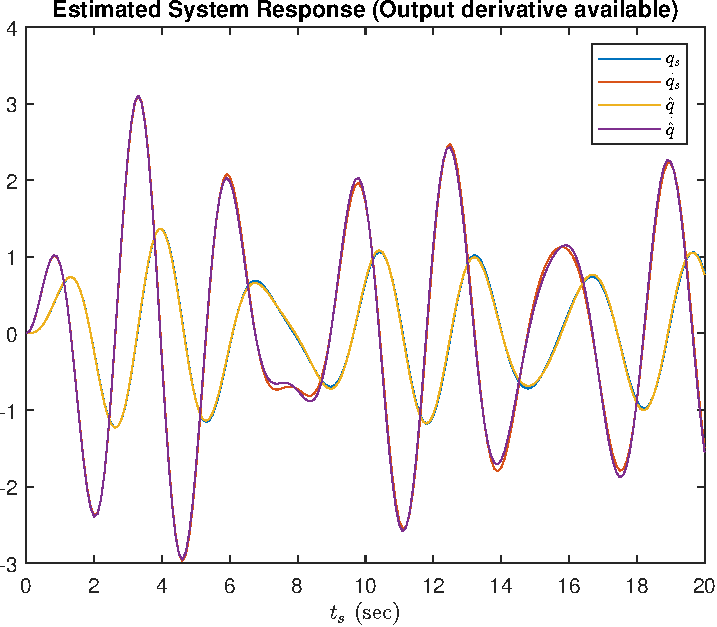
\includegraphics[width=\linewidth]{plot/task2_response_with_derivative.pdf}
        \caption{Απόκριση του εκτιμόμενου συστήματος με $\dot{q}(t)$ μετρήσιμο}
        \label{fig:task2_response_with_derivative}
    \end{minipage}
    \hfill
    \begin{minipage}{0.45\textwidth}
        \centering
        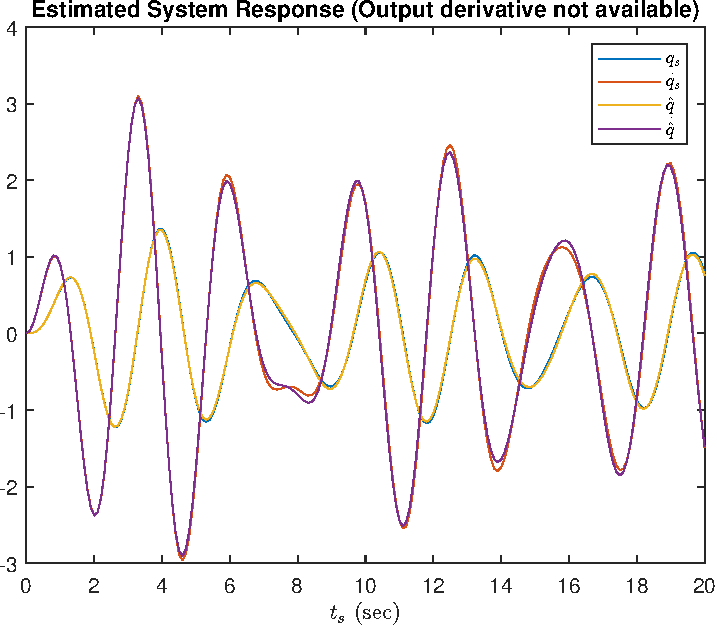
\includegraphics[width=\linewidth]{plot/task2_response_without_derivative.pdf}
        \caption{Απόκριση του εκτιμόμενου συστήματος με $\dot{q}(t)$ \textbf{μη} μετρήσιμο}
        \label{fig:task2_response_without_derivative}
    \end{minipage}
\end{figure}

\begin{figure}
    \centering
    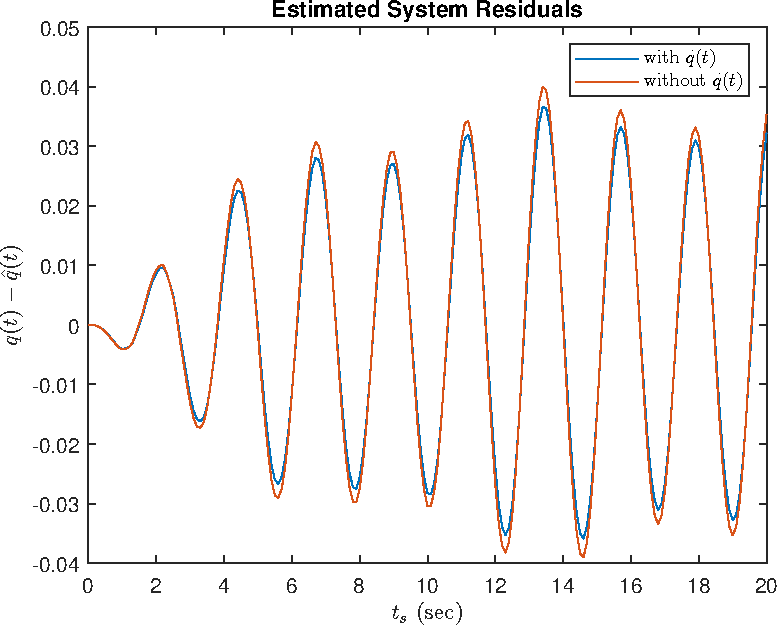
\includegraphics[width=0.5\linewidth]{plot/task2_residuals.pdf}
    \caption{Σφάλμα απόκρισης εκτιμόμενου συστήματος με και χωρίς την γνώση του $\dot{q}(t)$}
    \label{fig:task2_residuals}
\end{figure}

\subsection*{Ερώτημα 2β}

%%%%%%%%%%%%%%%%%%%%%%%%%%%%%%%%%%%%%%%%%%%%%%%%%%%%%%%%%%%%%%%%%%%%%%%%%%%%%%%%%%%%%%%%%%%%%%%%%%%%%%

Θα εκτιμήσουμε τις παραμέτρους $m, L, c$ του συστήματος θεωρώντας αυτή τη φορά ότι μετρήσιμα μεγέθη είναι μόνο η έξοδος
$q(t)$ και η είσοδος $u(t)$. Όπως και στην προηγούμενη περίπτωση, θα πρέπει να φέρουμε το σύστημα στην γραμμική 
παραμετροποιήσιμη μορφή. Θέτωντας στην (\ref{eq:linear_parametric_form}) $\ddot{q}(t) = s^2q, \, \dot{q}=sq$ και 
φιλτράροντας τα δύο μέλη της με ένα ευσταθές φίλτρο $\Lambda(s)  =s^2 + \lambda_1 s + \lambda_2$ παίρνουμε:
\begin{equation}
\begin{aligned}
    \frac{s^2}{\Lambda(s)}q &=
    \left[
    \begin{matrix}
        \frac{c}{mL^2} & \frac{g}{L} & \frac{1}{mL^2}
    \end{matrix}
    \right]
    \cdot
    \left[
    \begin{matrix}
        -\frac{sq}{\Lambda(s)} & -\frac{q}{\Lambda(s)} & \frac{u}{\Lambda(s)}
    \end{matrix}
    \right]^T 
    \implies \\
    \frac{\Lambda(s) - \lambda_1s-\lambda_2}{\Lambda(s)}q &=
    \left[
    \begin{matrix}
        \frac{c}{mL^2} & \frac{g}{L} & \frac{1}{mL^2}
    \end{matrix}
    \right]
    \cdot
    \left[
    \begin{matrix}
        -\frac{sq}{\Lambda(s)} & -\frac{q}{\Lambda(s)} & \frac{u}{\Lambda(s)}
    \end{matrix}
    \right]^T
    \implies \\
    \left(1 - \frac{\lambda_1s + \lambda_2}{\Lambda(s)}\right)q &=
    \left[
    \begin{matrix}
        \frac{c}{mL^2} & \frac{g}{L} & \frac{1}{mL^2}
    \end{matrix}
    \right]
    \cdot
    \left[
    \begin{matrix}
        -\frac{sq}{\Lambda(s)} & -\frac{q}{\Lambda(s)} & \frac{u}{\Lambda(s)}
    \end{matrix}
    \right]^T
    \implies \\
    q &=
    \left[
    \begin{matrix}
        \frac{c}{mL^2}-\lambda_1 & \frac{g}{L}-\lambda_2 & \frac{1}{mL^2}
    \end{matrix}
    \right]
    \cdot
    \left[
    \begin{matrix}
        -\frac{sq}{\Lambda(s)} & -\frac{q}{\Lambda(s)} & \frac{u}{\Lambda(s)}
    \end{matrix}
    \right]^T
    \implies \\
    q &= \theta^T \phi
    \label{eq:linear_parametric_form3}   
\end{aligned}
\end{equation}
Βλέπουμε ότι ο πίνακας οπισθοδρόμησης διάστασης περιλαμβάνει μόνο μετρήσεις εισόδου-εξόδου που είναι γνωστές,
συνεπώς μπορούμε να εκτιμήσουμε το $\theta$ με την μέθοδο των ελαχίστων
τετραγώνων από την σχέση:
\begin{equation}
    \theta = \left(\sum_{t=1}^N\phi^T(t)\phi(t)\right)^{-1}\sum_{t=1}^N\phi^T(t)q(t)
\end{equation}
Έχοντας εκτιμήσει το $\theta = [\theta_1 \quad \theta_2 \quad \theta_3]$, οι εκτιμήσεις των παραμέτρων $m, L, c$
δίνονται από:
\begin{equation}
    \begin{aligned}
        \hat{c} &= \frac{\theta_1 + \lambda_1}{\theta_3} \\
        \hat{L} &= \frac{g}{\lambda_2 + \theta_2} \\
        \hat{m} &= \frac{1}{\theta_3 \hat{L}^2}
    \end{aligned}
\end{equation}

Οι εκτιμήσεις των παραμέτρων και τα αντίστοιχα σχετικά σφάλματα δίνονται στον 
Πίνακα~\ref{tab:task2_estimations_without_derivative}. Παρατηρούμε οι εκτιμήσεις των
$m, L$ είναι ελάχιστα χειρότερες από την περίπτωση όπου το $\dot{q}$ είναι μετρήσιμο ενώ η εκτίμηση
του $c$ είναι ελαφρώς καλύτερη σε αυτή την περίπτωση. Αυτές οι τόσο μικρές διαφορές στην ακρίβεια συμβαίνουν
λόγω του πολύ μικρού βήματος ολοκλήρωσης που επιλέξαμε. Όπως θα δούμε στην συνέχεια, μεγαλύτερο βήμα ολοκλήρωσης
έχει ως αποτέλεσμα η εκτίμηση των παραμέτρων με γνώση του $\dot{q}(t)$ να δίνει σημαντικά καλύτερα αποτελέσματα από
την μη γνώση του.

\begin{table}[h!]
\centering
\begin{tabular}{|l|c|c|c|}
\hline
\multicolumn{1}{|c|}{} & \multicolumn{1}{c|}{$m$} & \multicolumn{1}{c|}{$c$} & \multicolumn{1}{c|}{$L$} \\
\hline
\textbf{εκτίμηση} & 0.752943 & 0.149748 & 1.240937 \\
\textbf{σχετικό σφάλμα (\%)} & 0.392387 & 0.167878 & 0.725018 \\
\hline
\end{tabular}
\caption{Εκτιμήσεις παραμέτρων με $\dot{q}(t)$ \textbf{μη} μετρίσιμο}
\label{tab:task2_estimations_without_derivative}
\end{table}

Στο Σχ.~\ref{fig:task2_response_without_derivative} βλέπουμε την απόκριση του συστήματος που προέκυψε από την
εκτίμηση των παραμέτρων $m, L, c$ σε σχέση με την απόκριση του αρχικού συστήματος. Παρατηρούμε και πάλι ότι το 
εκτιμόμενο σύστημα προσεγγίζει ικανοποιητικά την συμπεριφορά του αρχικού συστήματος με μέσο τετραγωνικό 
σφάλμα 0.021544. Στο Σχ.~\ref{fig:task2_residuals} παρατίθεται
η γραφική παράσταση του σφάλματος $e(t) = q(t) - \dot{q}(t)$. Παρατηρούμε ότι το πλατος του $e(t)$
για την περίπτωση όπου το $\dot{q}(t)$ δεν είναι μετρίσιμο είναι ελαφρώς μεγαλύτερο από την περίπτωση που το 
$\dot{q}(t)$ είναι μετρήσιμο. Αυτό εξηγείται από το γεγονός ότι στην πρώτη περίπτωση αξιοποιούμε την γνώση μας
για το $\dot{q}(t)$ οδηγόντας μας σε καλύτερα αποτελέσματα.

%%%%%%%%%%%%%%%%%%%%%%%%%%%%%%%%%%%%%%%%%%%%%%%%%%%%%%%%%%%%%%%%%%%%%%%%%%%%%%%%%%%%%%%%%%%%%%%%%%%%%%

\section*{Θέμα 3}

\subsection*{Ερώτημα 3α}

Σε αυτό το μέρος προσθέτουμε λευκό γκαουσιανό θόρυβο με τυπική απόκλιση 0.01 στα δεδομένα δειγματολειψίας και
εκτιμούμε τις παραμέτρους $m, c, L$ με και χωρίς την γνώση του $\dot{q}(t)$. Οι εκτιμήσεις των παραμέτρων και τα 
αντίστοιχα σχετικα τους σφάλματα φαίνονται στον Πίνακα~\ref{tab:task3_estimations_with_derivative_WGN} και 
Πίνακα~\ref{tab:task3_estimations_without_derivative_WGN}. Όπως ήταν αναμενόμενο,
οι εκτημήσεις μας είναι χειρότερες όταν προσθέτουμε λευκο θόρυβο στα δεδομένα δειγματολειψίας ενώ όσο μεγαλύτερη 
είναι η τυπική απόκλιση του θορύβου, τόσο χειρότερες γίνονται και οι εκτιμήσεις μας. Επίσης παρατηρούμε πως όταν
προσθέτουμε λευκό θόρυβο η γνώση του $\dot{q}(t)$ συνεισφέρει σηματικά στην καλή εκτίμηση των παραμετρων.

Στα Σχ.~\ref{fig:task3_response_with_derivative_WGN} έως Σχ.~\ref{fig:task3_residuals_without_derivative_WGN} φαίνεται
η επιδραση του θορύβου στις αποκρίσεις και τα σφάλματα του συστήματος που προκύπτει επειτα απο την εκτιμηση των παραμετρων.
Όπως είναι εμφανές η προσθεση θορυβου οδηγει σε μεγαλύτερο σφαλμα στην απόκριση του συστήματος.

\subsection*{Ερώτημα 3β}

Στο Σχ.~\ref{fig:task3_parameter_estimation_error_vs_sampling_period} βλέπουμε το σχετικό σφάλμα εκτίμησης παραμέτρων
συναρτήσει της περιόδου δειγματολειψίας $T_s$. Παρατηρούμε πως το σφάλμα αυξάνεται με την άυξηση της περιοδου 
δειγματολειψιας καθώς χάνουμε σε πληροφορία. Επίσης όσο μεγαλύτερο είναι το $T_s$ τόσο σημαντικότερη γίνεται η
επίδραση της γνώσης του $\dot{q}(t)$ στην καλή εκτίμηση των παραμέτρων

\begin{figure}
    \centering
    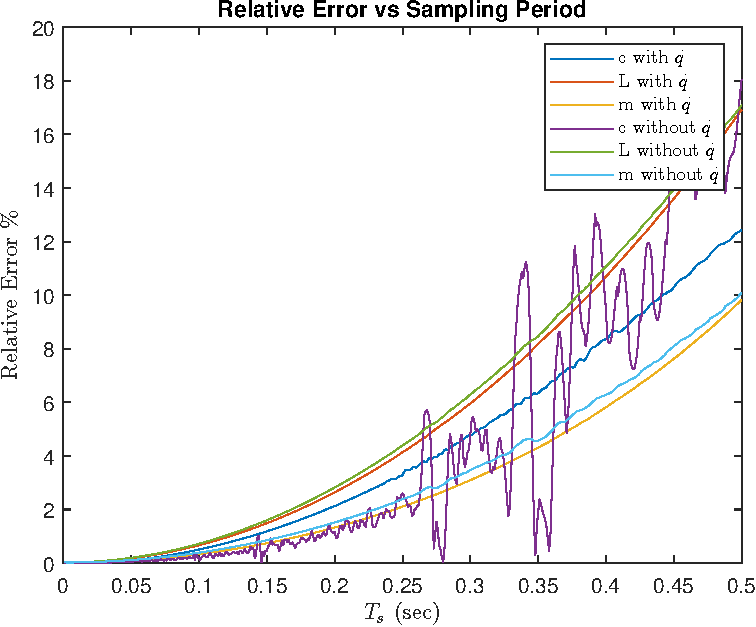
\includegraphics[width=0.5\linewidth]{plot/task3_parameter_estimation_error_vs_sampling_period.pdf}
    \caption{Σχετικό σφάλμα εκτίμησης παραμέτρων συναρτήσει της περιόδου δειγματολειψίας}
    \label{fig:task3_parameter_estimation_error_vs_sampling_period}
\end{figure}

\subsection*{Ερώτημα 3γ}

Στο Σχ.~\ref{fig:task3_parameter_estimation_error_vs_input_amplitude} βλέπουμε το σχετικό σφάλμα εκτίμησης παραμέτρων
συναρτήσει του πλάτους του σήματος εισόδου $A_0$. Παρατηρούμε πως το σφάλμα δεν μεταβάλλεται με την αύξηση του $A_0$
με εξαίρεση την παράμετρο $c$ όπου το σφάλμα της παρουσιάζει μεγάλες διακυμάνσεις.

\begin{figure}
    \centering
    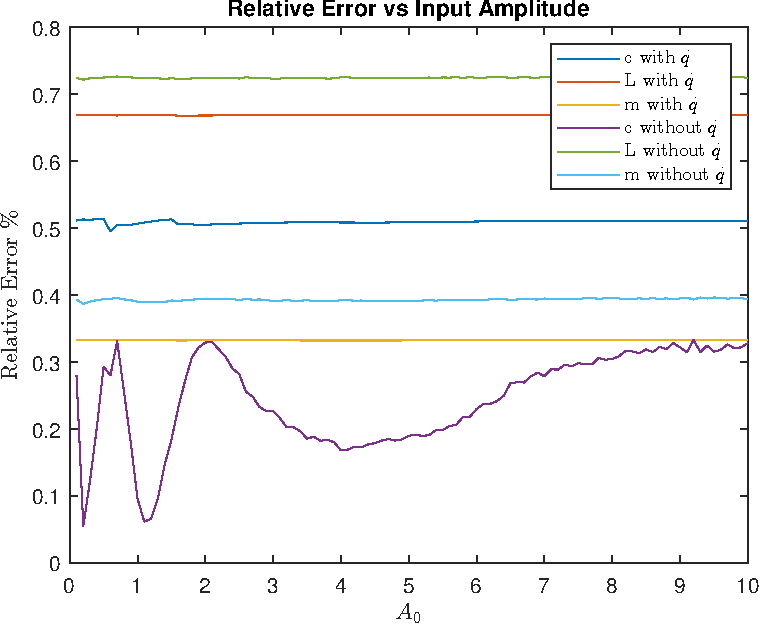
\includegraphics[width=0.5\linewidth]{plot/task3_parameter_estimation_error_vs_input_amplitude.pdf}
    \caption{σχετικό σφάλμα εκτίμησης παραμέτρων συναρτήσει του πλάτους του σήματος εισόδου $A_0$}
    \label{fig:task3_parameter_estimation_error_vs_input_amplitude}
\end{figure}

\begin{table}[h!]
\centering
\begin{tabular}{|l|c|c|c|}
\hline
\multicolumn{1}{|c|}{} & \multicolumn{1}{c|}{$m$} & \multicolumn{1}{c|}{$c$} & \multicolumn{1}{c|}{$L$} \\
\hline
\textbf{εκτίμηση} & 0.753437 & 0.154553 & 1.242763 \\
\textbf{σχετικό σφάλμα (\%)} & 0.458269 & 3.035263 & 0.578945 \\
\hline
\end{tabular}
\caption{Εκτιμήσεις παραμέτρων με $\dot{q}(t)$ μετρίσιμο και λευκό θόρυβο}
\label{tab:task3_estimations_with_derivative_WGN}
\end{table}

\begin{table}[h!]
\centering
\begin{tabular}{|l|c|c|c|}
\hline
\multicolumn{1}{|c|}{} & \multicolumn{1}{c|}{$m$} & \multicolumn{1}{c|}{$c$} & \multicolumn{1}{c|}{$L$} \\
\hline
\textbf{εκτίμηση} & 0.763004 & -0.347266 & 1.239204 \\
\textbf{σχετικό σφάλμα (\%)} & 1.733862 & 331.510390 & 0.863664 \\
\hline
\end{tabular}
\caption{Εκτιμήσεις παραμέτρων με $\dot{q}(t)$ \textbf{μη} μετρίσιμο και λευκό θόρυβο}
\label{tab:task3_estimations_without_derivative_WGN}
\end{table}


\begin{figure}[!h]
    \centering
    \begin{minipage}{0.45\textwidth}
        \centering
        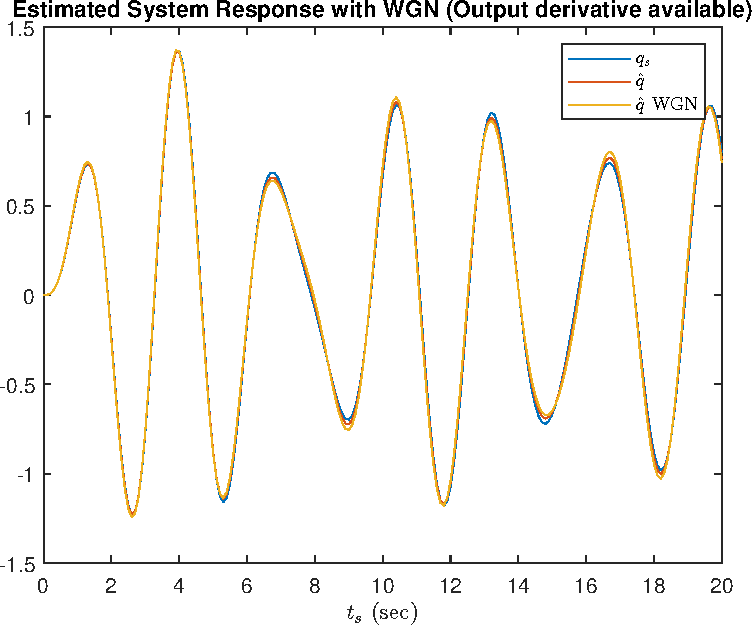
\includegraphics[width=\linewidth]{plot/task3_response_with_derivative_WGN.pdf}
        \caption{Απόκριση του εκτιμόμενου συστήματος με $\dot{q}(t)$ μετρήσιμο και λευκό θόρυβο}
        \label{fig:task3_response_with_derivative_WGN}
    \end{minipage}
    \hfill
    \begin{minipage}{0.45\textwidth}
        \centering
        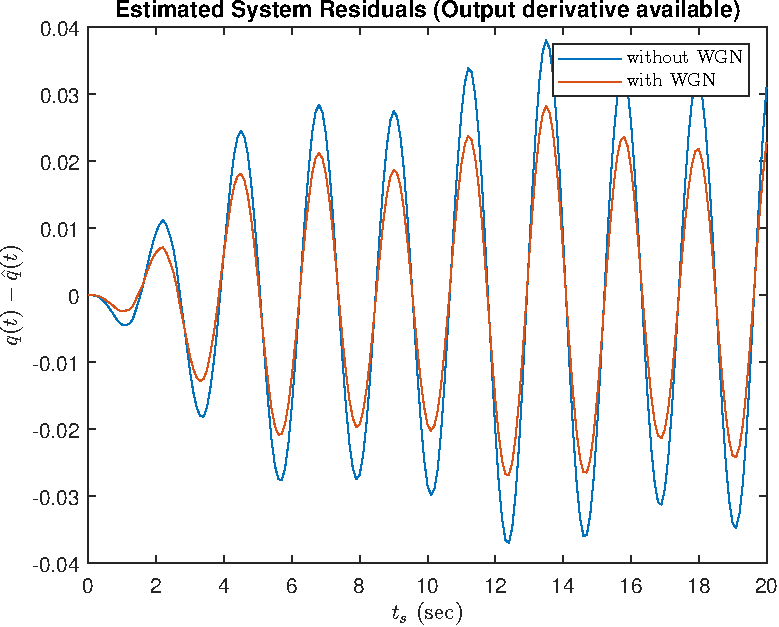
\includegraphics[width=\linewidth]{plot/task3_residuals_with_derivative_WGN.pdf}
        \caption{Σφάλμα εκτιμόμενου συστήματος με $\dot{q}(t)$ μετρήσιμο και λευκό θόρυβο}
        \label{fig:task3_residuals_with_derivative_WGN}
    \end{minipage}
\end{figure}

\begin{figure}[!h]
    \centering
    \begin{minipage}{0.45\textwidth}
        \centering
        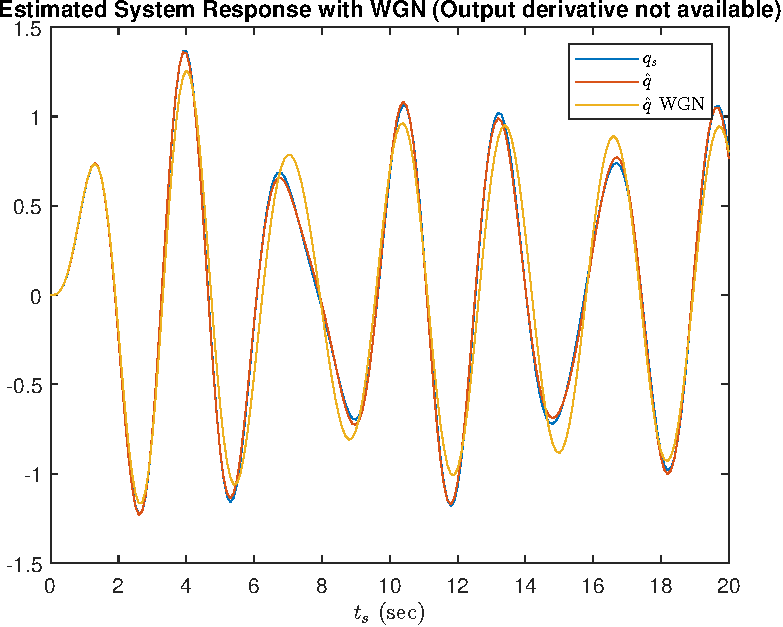
\includegraphics[width=\linewidth]{plot/task3_response_without_derivative_WGN.pdf}
        \caption{Απόκριση του εκτιμόμενου συστήματος με $\dot{q}(t)$ \textbf{μη} μετρήσιμο και λευκό θόρυβο}
        \label{fig:task3_response_without_derivative_WGN}
    \end{minipage}
    \hfill
    \begin{minipage}{0.45\textwidth}
        \centering
        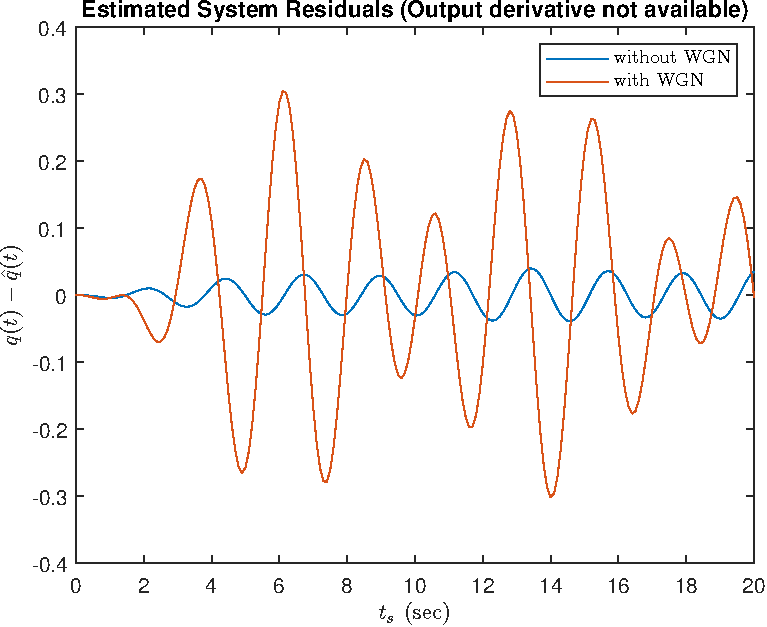
\includegraphics[width=\linewidth]{plot/task3_residuals_without_derivative_WGN.pdf}
        \caption{Σφάλμα εκτιμόμενου συστήματος με $\dot{q}(t)$ \textbf{μη} μετρήσιμο και λευκό θόρυβο}
        \label{fig:task3_residuals_without_derivative_WGN}
    \end{minipage}
\end{figure}

\end{document}
